\chapter{Hyperbolic geometry}\label{hyperbolic}
We introduce hyperbolic spaces by putting them in contrast with the Euclidean space we are more accustomed to. We then briefly discuss (Reimanninan) manifolds, which are the mathematical framework for hyperbolic spaces. In addition, using the lens of manifolds, we highlight some of characteristics of hyperbolic spaces. Lastly, leading up to \Cref{hrl}, we stress the connection between hyperbolic spaces and tree-like structures.

\section{Beyond Euclidean geometry}

\subsection{The parallel postulate}\label{sec:parallelPostulate}
In 300 BC Euclid wrote his \textit{Elements}, consisting of thirteen books (translated in~\cite{Fitzpatrick2008euclidElementsGeometry}). In the first book he spoke about five postulates which form the basis of Euclidean geometry. A literal translation of these the postulates (with the exception of the fifth) is:
\begin{enumerate}
    \item Let it have been postulated to draw a straight line from any point to any point.
    \item To produce a finite straight line continuously in a straight line.
    \item To describe a circle with any center and distance.
    \item That all right angles are equal to another.
    \item (Parallel Postulate) Through a point $P$ outside of an infinitely long line $\ell$ there is only one infinitely long line that does not cut the first line $\ell$.
\end{enumerate}

This Parallel Postulate is known as Playfair’s postulate, the most used alternative for Euclid’s real fifth postulate. The original fifth postulate states:
\begin{quote}
    That, if a straight line on two (other) straight lines makes the interior angles on the same side less than two right angles, the two straight lines, if produced indefinitely, meet on that side on which the angles are less than the two right angles.
\end{quote}


It is possible to obtain internally consistent models of geometries which obey to all postulates except for the parallel postulate. These geometries are denoted as \term{non-Euclidean geometries}. One way to do this might be to insist that any two lines intersect. This gives rise to so called \term{Elliptic Geometry}. Another way of obtaining a non-Euclidean geometry is to state that the line through point $P$ that does not meet $\ell$ is not unique. This determines \term{Hyperbolic Geometry}, in which the parallel postulate is replaced by the following.


\begin{postulate}(Hyperbolic parallel postulate)
    Given any line $\ell$ and a point $P$ not on $\ell$, there are at least two lines though $P$ that do not meet $\ell$. In other words there are at least two lines through $P$ that are parallel to $\ell$.
\end{postulate}


\begin{figure}
    \centering
    \begin{subfigure}{0.2\textwidth}
        \centering
        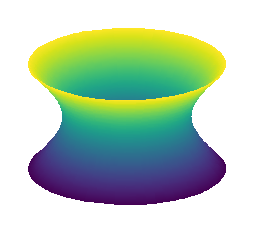
\begin{tikzpicture}[scale=0.5]
            \begin{axis}[
                    view={30}{30},
                    axis lines=none,
                    colormap/viridis,
                    samples=60,
                    domain=-1:1,
                    y domain=-2*pi:2*pi
            ]
            \addplot3[
                    surf,
                    shader=interp,
                    z buffer=sort
            ] ({0.2+cosh(x)*cos(deg(y))},
            {0.2+cosh(x)*sin(deg(y))},
            {sinh(x)});     
            \end{axis}
        \end{tikzpicture}
        \caption{Negative curvature}
     \end{subfigure}
     \hfill
     \begin{subfigure}{0.2\textwidth}
        \centering
        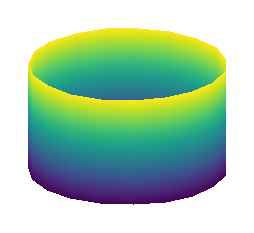
\begin{tikzpicture}[scale=0.5]
            \begin{axis}[
                    view={30}{30},
                    axis lines=none,
                    colormap/viridis,
                    samples=20,
                    domain=0:2*pi,
                    y domain=-1.5:1.5
            ]
            \addplot3[
                    surf,
                    shader=interp,
                    z buffer=sort
            ] ({cos(deg(x))},
            {sin(deg(x))},
            {y});
            \end{axis}
        \end{tikzpicture}
        \caption{Zero curvature.}
     \end{subfigure}
     \hfill
     \begin{subfigure}{0.2\textwidth}
        \centering
        
\begin{tikzpicture}[scale=0.5]
            \begin{axis}[
                    view={30}{0},
                    axis lines=none,
                    colormap/viridis,
                    samples=20,
                    domain=-90:90,
                    y domain=0:360
            ]
            \addplot3[
                    surf,
                    shader=interp,
                    z buffer=sort
            ]
            ({cos(x)*cos(y)},
            {cos(x)*sin(y)},
            {sin(x)});
            \end{axis}
        \end{tikzpicture}
        \caption{Positive curvature}     
    \end{subfigure}
    \label{fig:spaceCurvatures}\
    \caption{Surfaces with various curvatures.}
\end{figure}
Spaces in non-Euclidean geometries can be classified according to their curvature, which measures the deviation from flat Euclidean spaces. Specifically, spaces in elliptic geometry have positive curvature, whilst those in hyperbolic geometry possess negative curvature, as depicted in \Cref{fig:spaceCurvatures}. 

\subsection{Reimannian manifolds}
A Riemannian manifold is a mathematical space that generalizes the concept of curved surfaces and higher-dimensional spaces, allowing us to define distances, angles, and curvature in a smooth way. 

\begin{definition} (Reimannian manifold)
Given a smooth manifold $\Mcal$, a Riemannian metric is a smooth function that assigns to each $p \in \Mcal$ an inner product on the tangent space $\mathcal{T}_p\Mcal$:
\begin{equation*}
    g_p: \mathcal{T}_p\Mcal \times \mathcal{T}_athcal{T}_athcal{T}_athcal{T}_p\Mcal \to \R.
\end{equation*}
    A Reimannian manifold is a pair $(\Mcal,g)$ where $\Mcal$ is a smooth manifold and $g$ is a Riemannian metric.
\end{definition}

Simply put, a \term{manifold} is a topological space\footnote{A \term{topological space} is a set of points, along with a topology, an additional structure which can be defined as a set of neighbourhoods for each point that satisfy some axioms formalizing the concept of closeness.} that locally resembles Euclidean space near each point. More precisely, a $d$-manifold  is a topological space with the property that each point has a neighborhood that resembles an open subset of $d$-dimensional Euclidean space. 

A \term{smooth manifold} is such when functions and coordinate changes along the manifold are infinitely differentiable. The associated metric entails that at each point $p$ lengths and angles are measured differently. 

\paragraph{Distance function and geodesics} An important concept in Euclidean geometry, arising from Euclid's first postulate (\Cref{sec:parallelPostulate}), is that of straight lines, which are shortest paths between points. We can generalize this concept to manifolds by seeking curves with minimal length, called \term{geodesics}. A geodesic is a curve $\gamma(t)=(\gamma(t)^1, \dots, \gamma(t)^d)$ in a manifold $\Mcal$ connecting points $p,q\in \Mcal$ with minimum length. 

In Euclidean space geodesics are straight lines in $\R^d$ and for given parameters $a,b\in \R^d$ they have the form 
\begin{equation}
    \gamma(t) = t\cdot a + b.
\end{equation}

\paragraph{Exponential and logarithmic maps} We would like to associate the points in a manifold to those on a tangent Euclidean space. The tangent space maps to the manifold via an exponential map, and conversely, a logarithmic map translates a point on the manifold to the tangent space. We will see an example of these maps in the following section.

For more details on foundations of manifolds refer to the Appendix in~\cite{Chami2021representationLearningAlgorithmsHyperbolicSpaces}, or~\cite{doCarmo1992riemannianGeometry}\cite{Lee2003smooth}.


\section{Hyperbolic spaces}
Building on the concept of manifolds we analyze how distances and straight lines morph in hyperbolic spaces. In fact, in negative curvature spaces, the space bends like a saddle and triangle angles sum to less than $\pi$. As an example we show a section of a hyperbolic paraboloid (described by function $z=x^2-y^2$) in \Cref{fig:hyperbolicSpace}. In practice it would not be possible to work directly on hyperbolic spaces. Hence, we introduce some ways to operate on hyperbolic spaces and help in their representation. Hyperbolic spaces of constant curvature are difficult to envisage because they cannot be isometrically embedded into any Euclidean space. The reason is, informally, that the former are ``larger'' and have more ``space'' than the latter.  

Because of the fundamental difficulties in representing spaces of constant negative curvature as subsets of Euclidean spaces, there are many equivalent models of hyperbolic spaces\footnote{The possible models of hyperbolic spaces are the following: the Poincaré ball, the Poincaré half-ball, the Klein ball, the hyperboloid model and the upper half-space model.}. Each model emphasizes different aspects of hyperbolic geometry, but no model simultaneously represents all of its properties. In \Cref{sec:hyperboloidModel} we introduce the hyperboloid model as it is useful for computation due to relatively simple formulas for geodesics a. We then focus on Poincaré ball model in \Cref{sec:poincareBall}, that represents the infinite hyperbolic space in a finite ball, and is therefore very useful for visualizations. We then show the relation between these two models (\Cref{sec:isometry}).

For both the models we show how distances are measured and how minimum-length lines are defined. We also put in evidence the respective exponential and logarithmic maps that relate the points on the models to to tangent spaces which are vector spaces that are isomorphic to $\R^d$. In \Cref{hrl} we will use these maps to leverage some of the tools of Euclidean geometry in which standard operations like addition and multiplication are defined for hyperbolic methods, such as optimization or neural network operations.

More in depth discussion on hyperbolic geometry can be found in~\cite{Anderson2006hyperbolicGeometry}\cite{Ramsay2013introductionHyperbolicGeometry}.

\begin{figure}
    \centering
    \begin{tikzpicture}
        \begin{axis}[
            view={160}{70},
            colormap/viridis,
            shader=interp,
            axis lines=none,
            xmin=-2, xmax=2,
            ymin=-2, ymax=2,
            zmin=-2, zmax=2,
        ]
        
        % Plot the hyperbolic paraboloid
        \addplot3[
            surf,
            domain=-1.7:1.7,
            domain y=-2:1.5,
            samples=30,
            opacity=0.8,
        ] {x^2 - y^2};
        
        % Define vertices of the triangle (lying on the surface)
        \newcommand{\vertexA}{(-1, -1, 0)}    % z = (-1)^2 - (-1)^2 = 0
        \newcommand{\vertexB}{(1, -1, 0)}     % z = 1^2 - (-1)^2 = 0
        \newcommand{\vertexC}{(0, 1, -1)}     % z = 0^2 - 1^2 = -1
        
        % Edge from A to B (along y = -1, z = x^2 - 1)
        \addplot3[
            thick,
            red,
            smooth,
            samples=50,
            samples y=0,
            domain=-1:1,
        ] ( 
            {x},                % x(x) = -1 → 1
            {-1},               % y(x) = -1 (consxanx)
            {x^2 - 1}         % z(x) = x(t)^2 - y(t)^2 = t^2 - 1
        );
        
        % Edge from A to C (parametric curve)
        \addplot3[
            thick,
            red,
            smooth,
            samples=50,
            samples y=0,
            domain=0:1,
        ] ( 
            {-1 + x},           % x(x) = -1 → 0
           { -1 + 2*x},         % y(x) = -1 → 1
            {(-1 + x)^2 - (-1 + 2*x)^2}  % z(x) = x(t)^2 - y(t)^2
        );
        
        % Edge from B to C (parametric curve)
        \addplot3[
            thick,
            red,
            smooth,
            samples=50,
            samples y=0,
            domain=0:1,
        ] ( 
            {1 - x},            % x(x) = 1 → 0
            {-1 + 2*x},         % y(x) = -1 → 1
            {(1 - x)^2 - (-1 + 2*x)^2}  % z(x) = x(t)^2 - y(t)^2
        );
        \end{axis}
        \end{tikzpicture}

    % 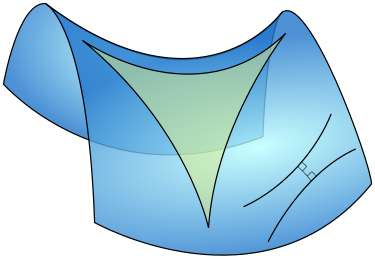
\includegraphics[width=0.3\textwidth]{figs/Hyperbolic_triangle.png}    
    \caption{Section of a hyperbolic space.}
    \label{fig:hyperbolicSpace}
\end{figure}




\subsection{Hyperboloid model}\label{sec:hyperboloidModel}
We first introduce some useful quantities for our discussion.

\begin{definition}(Minkowski inner product) \label{def:minkowskiInnerProduct}
    Given two vectors $x,y \in \R^d$, their Minkowski inner product is defined as:
    \begin{equation*}
        \langle x, y \rangle_\Lcal = -x_0y_0+\sum_{i=1}^d x_iy_i
    \end{equation*}    
\end{definition}

\begin{definition}(Minkowski norm) \label{def:minkowskiNorm}
    Given a vector $x \in \R^d$, its Minkowski norm is defined as:
    \begin{equation*}
        \|x\|_\Lcal = \sqrt{\langle x, x \rangle_\Lcal}.
    \end{equation*}
\end{definition}

We can now define the hyperboloid model of hyperbolic space.
\begin{definition}[Hyperbolic model]
    We denote $\Hy^{d,\kappa}$ as the hyperboloid manifold in $d$ dimension with constant negative curvature $\frac{1}{\kappa}$ with $\kappa>0$ as
    \begin{equation*}
        \Hy^{d,\kappa} = \left\{x \in \R^{d+1} : \langle x, x \rangle_\Lcal = -\kappa, x_0 > 0\right\}
    \end{equation*}
\end{definition}

\begin{figure}
    \begin{subfigure}{0.48\textwidth}
        \centering
        \begin{tikzpicture}[scale=1.7]
            \draw (0,0) circle (1);
            \clip (0,0) circle (1);
            \hgline{30}{-30}{black!70}
            \hgline{180}{270}{blue!20}
            \hgline{30}{120}{black!70}
            \hgline{0}{180}{red!50}
        \end{tikzpicture}
        \caption{Poincaré ball model.}
        \label{fig:poincareBall}
    \end{subfigure}%
    \hfill
    \begin{subfigure}{0.48\textwidth}
        \centering
        \begin{tikzpicture}
        \begin{axis}[
            view={30}{10},
            colormap name=custom,
            shader=interp,
            axis lines=none,
            xmin=-3, xmax=3,
            ymin=-3, ymax=3,
            zmin=0, zmax=5,
        ]
        \addplot3[
            surf,
            domain=-2.8:2.8,
            y domain=-2.8:2.8,
            samples=20,
            z buffer=sort,
            opacity=0.7
        ] {sqrt(x^2 + y^2 + 1)};
        \end{axis}
        \end{tikzpicture}   
        \caption{Hyperboloid model.}
        \label{fig:hyperboloid}
    \end{subfigure}
    \caption{Models of hyperbolic space.}
    \label{fig:hyperbolicmodels}
\end{figure}


For each point $p$ in a hyperboloid $\Hy^{d,\kappa}$ the tangent space at $p$---$\mathcal{T}_athcal{T}_p\Hy$---is a $d$-dimensional vector space containing all possible directions of paths leaving from $p$. Formally the tangent space to point $p$ is described as:
\begin{align*}
    \mathcal{T}_athcal{T}_athcal{T}_p\Hy^{d,\kappa} 
    &= \left\{u\in \R^{d+1} : \langle u, p \rangle_\Lcal = 0\right\} \\
    &= \left\{(v_0,v) \in \R^{d+1} : v_0 = \frac{v \cdot p}{\sqrt{\kappa(1 + \|p\|^2_2)}}\right\}
\end{align*}

From hereon we refer to a hyperboloid model with negative curvature $1$ ($\Hy^{d,1}$), that we simply indicate with $\Hy^d$. In two dimensions the hyperboloid can be visualized as a surface in $\R^3$ which corresponds to the upper sheet of a two sheet hyperboloid of revolution (\Cref{fig:hyperboloid}).

\paragraph{Distance function and geodesics}
Let $p\in\Hy^d$ and $v\in \mathcal{T}_athcal{T}_p\Hy^d$, assuming $\langle v,v\rangle_\Lcal $ = 1. In the hyperboloid model the unique geodesic $\gamma_{p,v}(\cdot)$ such that $\gamma_{p,v}(0)=p$ and $\dot{\gamma}_{p,v}(0)=v$ is given by:

\begin{equation*}
    \gamma_{p,v}(t) = \cosh(t)p + \sinh(t)v.
\end{equation*}

The corresponding intrinsic distance\footnote{An \term{intrinsic distance} refers to the shortest path between two points measured \emph{within} a given space or surface, rather than through an external surrounding space.} between two points $p,q\in\Hy^d$ can be computed as:

\begin{equation}\label{eq:distance_hyperboloid}
    d_{\Hy^d}(p, q) = \text{arcosh}(-\langle p, q \rangle_\Lcal).
\end{equation}

\paragraph{Exponential and logarithmic maps}
When dealing with the hyperboloid model, given $p \in \Hy^d$ and a tangent vector $v \in \mathcal{T}_p\Hy^d$, the exponential map $\exp_p: \mathcal{T}_p\Hy^d \to \Hy^d$ assigns to $v$ the point $\exp_p(v) := \gamma(1)$, where $\gamma$ is the unique geodesic satisfying $\gamma(0) = p$ and $\dot{\gamma}(0) = v$. The logarithmic map $\log_p: \Hy^d \to \mathcal{T}_pHy^d$ reverses back to the tangent space at $p$ such that $\log_p(\exp_p(v)) = v$. In hyperbolic spaces these operations form a bijection between the entire hyperbolic space and the tangent space at a point. The analytic expressions for the exponential and logarithmic maps are given below, under the assumption that $v\neq 0$.

\begin{align}
    \exp_p(v) &= \cosh(\|v\|_\Lcal)p + \sinh(\|v\|_\Lcal) \frac{v}{\|v\|_\Lcal} \label{eq:log_hyperboloid}\\
    \log_p(y) &= d_{\Lcal}(p,y)\frac{y + \langle p,y \rangle_{\Lcal}p}{\|y + \langle p,y \rangle_{\Lcal}p\|_{\Lcal}} \label{eq:exp_hyperboloid}
\end{align}

\subsection{Poincaré ball model}\label{sec:poincareBall}
Poincaré's representation of hyperbolic geometry is based on the points in the unit ball in $d$ dimensions, formally described as
\begin{equation*}
    \B^d = \{x \in \R^d: \|x\|^2_2 < 1\}.
\end{equation*}
The boundary of the ball is not a part of the hyperbolic plane it represents, but represents its infinitely remote points, called \term{boundary at infinity}.

We now use the mathematical framework called \term{gyrovector spaces}~\cite{ungar2022gyrovectorSpaceHyperbolicGeometry}\cite{Ungar1999HyperbolicPythagoreanTheoremPoincareDiscModel} to describe elementary operations such as additions and scalar multiplications in the Poincaré ball model in analogy with Euclidean geometry.

Vector addition is not well-defined in the hyperbolic space, since adding two points in the Poincaré ball might result in a point outside the ball. Instead, Möbius addition provides an analogue to Euclidean addition for hyperbolic space. We define the Möbius addition in the Poincaré ball model.

\begin{definition}[Möbius addition]
    Given two points $p,q\in\B^d$, the Möbius addition is defined as:
    \begin{equation*}
        p \oplus q = \frac{(1 +  2\langle p,q\rangle_2 + \|q\|^2_2)}{(1 + 2\langle p,q\rangle_2 + \|p\|^2_2\|q\|^2_2)}.
    \end{equation*}
    
\end{definition}

In contrast to Euclidean addition, it is neither commutative nor associative. However, it provides an analogue through the lens of the parallel transport concept. Given two points $x,y$ and a tangent vector $v$ in $\mathcal{T}_x$, there is a unique tangent vector in $\mathcal{T}_y$ which creates the same angle as $v$ with the direction of the geodesic connecting $x$ and $y$. This is called the \term{parallel transport} $P_{x\to y} (v)$ of $v$ along the geodesic from $x$ to $y$. In Euclidean geometry parallel transport is the standard Euclidean addition. Analagously, the Möbius addition satisfies the following property:
\begin{equation*}
    p\oplus q=\exp_{x}(P_{o\to x}(\log_o(q))).
\end{equation*}

Similarly, the Möbius scalar multiplication provides a way to scale points on a manifold by a scalar. In the case of the Poincaré ball it is defined as follows.

\begin{definition}[Möbius scalar multiplication]
    Given a point $p\in\B^d$ and a scalar $\alpha\in\R$, the Möbius scalar multiplication is defined as:
    \begin{equation*}
        \alpha \otimes p = \tanh({\alpha \tanh^{-1}(\|p\|_2)})\frac{p}{\|p\|^2_2}.
    \end{equation*}
\end{definition}

\paragraph{Distance function and geodesics}
When the unit ball is endowed with the family of inner products
\begin{equation*}
    g_p = \left(\frac{2}{1-\|p\|^2_2}\right)^2\mathbb{I}_d,
\end{equation*}
the pair $(\B^d,g)$ forms a Riemannian manifold of constant negative curvature. The induced distance between two points $p,q$ in $\B^d$ can be found through
\begin{align}\label{eq:poincareDistance}
    d_\B(p,q) &= \text{arcosh}\left(1 + 2\frac{\|p-q\|^2_2}{(1-\|p\|^2_2)(1-\|q\|^2_2)}\right)\\
              &= 2\text{arctanh}(\|-p\oplus q\|).
\end{align}

This yields geodesics that are either straight lines that go through the origin of the ball, or segments of circles that are perpendicular to the boundary of the ball as shown in \Cref{fig:hyperbolicmodels}. Using Möbius addition and scalar multiplication we can determine the geodesic between two points $p,q\in\B^d$ as follows:
\begin{equation*}
    \gamma_{p,q}(t) = p\oplus (-p \oplus y) \otimes t.
\end{equation*}

\paragraph{Exponential and logarithmic maps}\label{sec:expLogMaps_poincareBall}
Like for the hyperboloid model there exist analytical expressions that define the exponential and logarithmic maps in a given point $p$ lying on $\B^d$ and on the tangent space in that point $\mathcal{T}_p\B^d$. 

\begin{align}
    \exp_p(v) &= p \oplus \left(\tanh\left(\frac{\lambda_p\|v\|_2}{2}\right)\frac{v}{\|v\|_2}\right) \label{eq:exp_poincareBall} \\
    \log_p(y) &= \frac{2}{\lambda_p}\text{arctan}(\|-p \oplus y\|_2)\frac{-p \oplus y}{\|-p \oplus y\|_2} \label{eq:log_poincareBall}
\end{align}

where $\lambda_p$ is a curvature-dependent conformal factor at $p$.

\begin{figure}
  \centering
  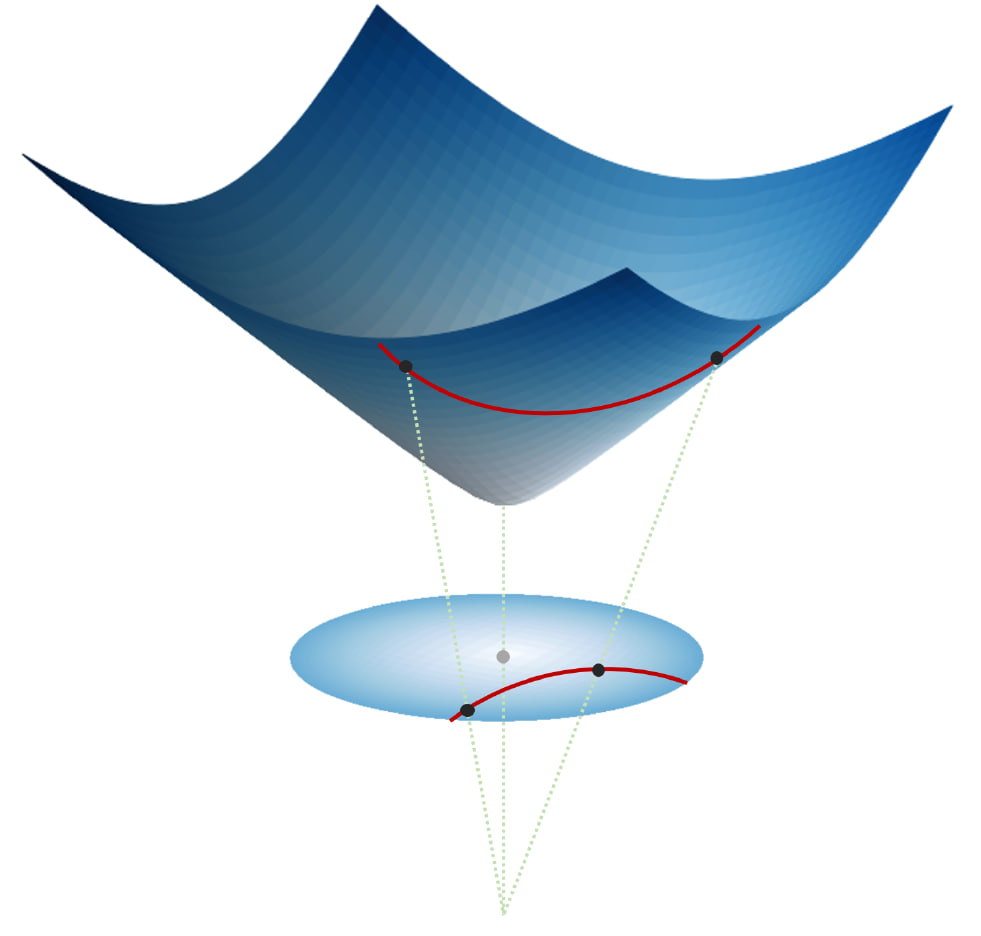
\includegraphics[width=0.5\textwidth]{figs/hyperboloidToPoincare.jpg}

    % \begin{tikzpicture}
    %     \begin{axis}[view={30}{20},axis lines=none]
    %       % Draw the hyperboloid
    %       \addplot3[surf, shader=interp, colormap/blackwhite, domain=-2:2]
    %         {x^2+y^2+1};
        
    %     % Limit geodesic curve to fit within the drawn hyperboloid
    %     \addplot3[domain=-0.9:1.63,samples=50, samples y=0, thick, blue]
    %     {sqrt(sinh(x)^2 + cosh(x)^2 + 1)+1};

        
          
    %     \end{axis}


    %   \end{tikzpicture}
  \caption{Illustration of the hyperboloid (top) and its connection to the Poincaré disk (bottom)\cite{Chami2021representationLearningAlgorithmsHyperbolicSpaces}.}
  \label{fig:hyperboloidToPoincareBall}
\end{figure}

\subsection{Isometry between hyperboloid and Poincaré ball}\label{sec:isometry}
The Poincaré ball model of hyperbolic space is isomorphic\footnote{An \term{isomorphism} is a bijective mapping between two structures that preserves their operations, relationships and properties.} to the hyperboloid model, as show in \Cref{fig:hyperboloidToPoincareBall}. The stereographic projection\footnote{The \term{stereographic projection} is a mapping that projects a sphere (space) onto a plane, preserving shapes locally.}
\begin{equation}\label{eq:stereographicProjection}
    (x_0, x_1, \ldots, x_d) \mapsto \left(\frac{x_1, \ldots, {x_d}}{1+x_0}\right)
\end{equation}
is an isometry between $\Hy^{d}$ and the Poincaré ball $\B^{d+1}$. Its inverse map is given by
\begin{equation}\label{eq:inverseStereographicProjection}
    (y_1, \ldots, y_d) \mapsto \left(\frac{1 + \|y\|^2, 2y_1, \ldots, 2y_d}{1 - \|y\|^2}\right).
\end{equation}

\section{Connections between hyperbolic spaces and trees}\label{sec:hyperbolicAndTrees}
We now discuss the connections between hyperbolic spaces and tree-like structures, that motivate the use of hyperbolic spaces to represent hierarchical data, as we will discuss in \Cref{hrl}. Various studies have shown that many real-world networks exhibit hierarchical structures with underlying hyperbolic geometry~\cite{Krioukov2010HyperbolicGeometryComplexNetworks}\cite{Papadopoulos2012popularityVSSimilarityGrowingNetworks}. We explore this relation theoretically by correlating hyperbolic metrics and tree metrics (\Cref{sec:hyperbolicTreeMetrics}), and more intuitively looking at the structure of trees (\Cref{sec:expGrowth}).

\subsection{Hyperbolic and tree metrics}\label{sec:hyperbolicTreeMetrics}
To identify tree-like structures we turn to notion of Gromov $\delta$-hyperbolicity~\cite{gromov1987hyperbolic}\cite{adcock2013tree}\cite{chen2013hyperbolicity}. To define $\delta$-hyperbolic spaces we introduce the Gromov product~\cite{gromov1987hyperbolic}. This quantity measures how close two points are to each other relative to a third point.  

\begin{definition}[Gromov product]
    In any metric space $(X,d)$, the Gromov product of two points $x,y\in X$ with respect to a third point $z\in X$ is defined as:
    \begin{equation*}
        \langle x,y \rangle_z = \frac{1}{2}\left(d(x,z) + d(y,z) - d(x,y)\right).
    \end{equation*}
\end{definition}

\begin{definition}[$\delta$-hyperbolicity, four-point condition]
    A metric space $(X,d)$ is $\delta$-hyperbolic if there exists $\delta\geq0$ such that for all $x,y,z,w\in X$
    \begin{equation*}
        \langle x,y\rangle_z \geq \min\{\langle x,w\rangle_z, \langle y, w\rangle_z\} - \delta.
    \end{equation*}
\end{definition}

We use a metric describing distances in trees as a baseline to compare metric spaces' $\delta$-hyperbolicities.

\begin{definition}[Metric tree]
    A metric space $(X,d)$ is a metric tree if there exists a tree $T=(X,E_T)$ with edges in $E_T$ such that for $u,v\in X$ it holds that $d(u,v)=d_T(u,v)$
\end{definition}
where $d_T(u,v)$ is the length of the shortest path between $u$ and $v$ in the tree $T$. 
 
\begin{figure}
    \centering
    \begin{tikzpicture}
        \node at (0,-1) [circle, draw, fill=black, inner sep=1pt] (z) {};
        \node at (0,-1.7) [circle, draw, fill=black, inner sep=1pt] (a) {};
        \node at (0,-2.4) [circle, draw, fill=black, inner sep=1pt] (b) {};
        \node at (-0.7,-3) [circle, draw, fill=black, inner sep=1pt]  (x) {};
        \node at (0.7,-3) [circle, draw, fill=black, inner sep=1pt] (c) {};
        \node at (1.4,-3.6) [circle, draw, fill=black, inner sep=1pt] (y) {};

        \draw[thick] (z) -- (a);
        \draw[thick] (a) -- (b);
        \draw[thick] (b) -- (x);
        \draw[thick] (b) -- (c);
        \draw[thick] (c) -- (y);

        \draw [decorate,decoration={brace,amplitude=8pt,mirror}] (b) -- (z) node[midway,xshift=10pt,right]{\footnotesize $\langle x,y\rangle_z$};


        \node[left=0.1cm of z] {$z$};
        \node[left=0.1cm of x] {$x$};
        \node[right=0.1cm of y] {$y$};
        

    \end{tikzpicture}
    \caption{Interpretation of the Gromov product in a simple tree.}
    \label{fig:slimTriangle}
\end{figure}


\begin{figure}
    \begin{subfigure}{0.25\textwidth}
        \centering
        \begin{tikzpicture}
            \node at (0,1) [circle, draw, fill=black, inner sep=0.5pt] (z) {};
            \node at (-0.866,-0.5) [circle, draw, fill=black, inner sep=0.5pt]  (x) {};
            \node at (0.866,-0.5) [circle, draw, fill=black, inner sep=0.5pt] (y){};

            
            \draw (z) -- (x);
            \draw (y) -- (x);
            \draw (z) -- (y);

            \clip (0,0) circle (1);
        \end{tikzpicture}
        \caption{In a Euclidean space.}
    \end{subfigure}
    \hfill
    \begin{subfigure}{0.25\textwidth}
        \centering
        \begin{tikzpicture}
            \node at (0,1) [circle, draw, fill=black, inner sep=0.5pt] (z) {};
            \node at (-0.866,-0.5) [circle, draw, fill=black, inner sep=0.5pt] (x) {};
            \node at (0.866,-0.5) [circle, draw, fill=black, inner sep=0.5pt] (y) {};
                        
            \clip (0,0) circle (1);
            \hgline{90}{-30}{black};
            \hgline{-150}{-30}{black};
            \hgline{210}{90}{black};

        \end{tikzpicture}
        \caption{In a hyperbolic space.}
    \end{subfigure}
    \hfill
    \begin{subfigure}{0.25\textwidth}
        \centering
        \begin{tikzpicture}
            \node at (0,1) [circle, draw, fill=black, inner sep=0.5pt] (z) {};
            \node at (0,0.2) [circle, draw, fill=black, inner sep=0.01pt] (b) {};           
            \node at (-0.866,-0.5) [circle, draw, fill=black, inner sep=0.5pt]  (x) {};
            \node at (0.866,-0.5) [circle, draw, fill=black, inner sep=0.5pt] (y){};
            
            \draw (z) -- (b);
            \draw (b) -- (x);
            \draw (b) -- (y);

            \clip (0,0) circle (1);
        \end{tikzpicture}
        \caption{In a tree space.}
    \end{subfigure}
    \caption{Triangles in various metric spaces.}
    \label{fig:triangles}
\end{figure}
One can show that metric trees are $0$-hyperbolic. Let $(X,d)$ be a metric tree, then $\langle x, y\rangle_z$ is the maximum number of edges in $T=(X,E_T)$ between the node $z$ and a common parent for $x$ and $y$ (\Cref{fig:slimTriangle}). It follows that for $x,y,w\in X$ it holds that $\langle x,y\rangle_z \geq \min\{\langle x,w\rangle_z, \langle y, w\rangle_z\}$. Therefore, metric spaces with smaller $\delta$ will be closer to a tree metric. One can show that the Euclidean space is not $\delta$-hyperbolic, whilst hyperbolic spaces are $\log 3$-hyperbolic in the sense of Gromov. This can be noticed by observing triangles in a Euclidean, a hyperbolic and a tree metric (\Cref{fig:triangles}). Indeed we see that with lower $\delta$-hyperbolicity of the metric space, the distance between two vertices increasingly approaches the distance to the ``centre'' of the triangle.

There are important properties such as quasi-isometries between $\delta$-hyperbolic spaces and tree metric spaces. We formalize that any finite set of points in a $\delta$-hyperbolic space can be embedded in a tree metric with bounded distortion~\cite{gromov1987hyperbolic}.

\begin{proposition}[Tree-likeliness of hyperbolic space]
    There is a constant $C_n =\delta \cdot O(n)$ such that for any set of points $x_1, x_2, \dots,x_n$ in a $\delta$-hyperbolic space $(\Mcal,d_\Mcal)$ can be embedded via $f:\Mcal \to T$ into a tree metric $(T,d_T)$ such that:
    \begin{equation*}
        d_\Mcal(x_i, x_j)\leq d_T(f(x_i), f(x_j)) \leq d_\Mcal(x_i, x_j) + C_n.
    \end{equation*}
\end{proposition}

More specifically, Sarkar~\cite{sarkar2011lowDIstortionDelaunayEmbedding} derived a construction to embed trees in hyperbolic spaces with arbitrarily low-distortion in two dimensions.

\begin{proposition}[Sarkar]
    Any tree $T=(X,E_T)$ can be embedded into $(\mathbb{B}^2, d_\mathbb{B})$ with scale $\zeta = O(1/\varepsilon)$ and worst-case distortion at most $1 + \varepsilon$.
\end{proposition}

These nice quasi-isometries between hyperbolic spaces and tree metric spaces motivate the use of hyperbolic geometry to embed tree-like graphs with low distortion. Since we have these quasi-isometric mappings, hyperbolic spaces can be thought of as some continuous version of trees. We will leverage these properties in the next chapter. 

\subsection{Exponential volume growth}\label{sec:expGrowth}
As we have concluded in the previous section, trees can be thought of as the discrete approximation of some underlying hyperbolic space, where geodesics resemble shortest paths in discrete trees. One can define a notion of volume in trees as the number of nodes contained within some bounded distance (the radius) to the root of the tree. This volume grows exponentially as we increase the radius, as shown in \Cref{fig:radialTree}.

\tikzset{level 1/.style={sibling angle=60,level distance=32mm}}
\tikzset{level 2/.style={sibling angle=35,level distance=16mm}}
\tikzset{level 3/.style={sibling angle=20,level distance=8mm}}
\tikzset{every node/.style={circle, fill=black, inner sep=0pt, color=black}}
\tikzset{edge from parent/.style={segment angle=10,draw}}


\begin{figure}
    \centering
    \begin{tikzpicture}
    [grow cyclic, scale=0.35]
    \node {} 
    child  foreach \A in {1,1,1,1,1,1}{  
    node{} 
        child foreach \B in {2,2,2}{ 
        node {} 
            child foreach \C in {3,3,3}{
            node {} }
        }
    };
    \end{tikzpicture}
    \caption{Volume growth in trees.}
    \label{fig:radialTree}
\end{figure}


In Euclidean space the volume of balls grows polynomially with the radius, making it less suitable to represent exponentially growing graphs like trees. More concretely, because the growth is not as fast as that of the graph, the Euclidean space quickly becomes too crowded, resulting in geodesics intersecting each other.

In contrast, $\delta$-hyperbolic spaces, and in particular hyperbolic spaces, have exponential growth. For instance, in a two dimensional hyperbolic space with constant curvature $\kappa = -1$, the length of a circle is given as $2\pi \sinh r$ while the area of a ball is given as $2\pi(\cosh r - 1)$. Since $\sinh r = \frac{1}{2} (e^r - e^{-r})$ and $\cosh r = \frac{1}{2} (e^r + e^{-r})$, both disc area and circle length grow exponentially with $r$. 

This feature yields more room to fit complex hierarchies and makes these spaces ideal candidates to embed trees while accommodating for their exponential volume growth. 